\documentclass[12pt]{article} 
\usepackage[pdftex]{graphicx}
\usepackage{subfigure}
\usepackage{nicefrac}
\usepackage{geometry, amsmath, amssymb, array, cite, caption, float}
\setlength{\parindent}{0pt} 
\setlength{\parskip}{2ex}
\bibliographystyle{apalike} %unsrt} 
\begin{document} 
\title{Assessment of optical CT as a future QA tool for synchrotron x-ray microbeam therapy } 
\author{Ciara McErlean}
%\date{23/1/13} 
%\maketitle 
%\begin{abstract} 
%Synchrotron microbeam radiation therapy (MRT) is an advanced form of radiotherapy for which it is extremely difficult to provide adequate quality assurance. This may delay or limit its clinical uptake, particularly in the paediatric patient populations for whom it could be especially suitable. This study investigates the extent to which new developments in 3-D dosimetry using optical computed tomography (CT) can visualise MRT dose distributions, and assesses what further developments are necessary before fully quantitative 3-D measurements can be achieved. 
%Two experiments are reported. In the first cylindrical samples of the radiochromic polymer PRESAGE® were irradiated with different complex MRT geometries including multiport treatments of collimated ‘pencil’ beams, interlaced microplanar arrays and a multiport treatment using an anthropomorphic head phantom. Samples were scanned using transmission optical CT. In the second experiment, PVDR measurements using optical CT were compared with expected values from Monte Carlo simulations. The depth-of-field (DOF) of the optical CT system was characterised using a knife-edge method and the possibility of spatial resolution improvement through deconvolution of a measured point spread function (PSF) was investigated. 
%3-D datasets from the first experiment revealed excellent visualisation of the 50 µm beams and various discrepancies from the planned delivery dose were found. The optical CT PVDR measurements were found to be consistently 30\% of the expected Monte Carlo values and deconvolution of the microbeam profiles was found to lead to increased noise. The reason for the underestimation of the PVDR by optical CT was attributed to lack of spatial resolution, supported by the results of the DOF characterisation. 
%Solutions are suggested for the outstanding challenges and the data are shown already to be useful in identifying potential treatment anomalies.
%\end{abstract} 
%\newpage
%\tableofcontents 

\section{Introduction}
\label{sec:intro}


Synchrotron microbeam radiation therapy (MRT) is an advanced form of external beam radiotherapy treatment. It exploits the remarkable tolerance healthy tissue has for high doses of radiation when the doses are `spatially fractionated', that is, confined to a set of spatially separated regions each of very small volume. The effects of such radiation are strongly dependent on the geometry of the regions exposed and, in particular, on the width of the incident beam of radiation \cite{brauer-krischeffects2010}. It is hypothesised that, although normal tissue in the beam path is destroyed, regeneration of blood vessels across the ablated region is possible providing the beam width is sufficiently small and the `valley dose' sufficiently low. By contrast, tumour microvasculature seems less able to repair the damage caused. Although the molecular mechanisms of this selective radiovulnerability remain under investigation, the clinical potential of microbeam therapy is clear \cite{crosbie2010tumor} and there are early indications that such methods may also be useful in the treatment of other, non-cancerous diseases \cite{pouyatos2013synchrotron}.

Despite the many advantages of MRT and our increasing ability to administer it safely, it is still extremely difficult to verify that the planned dose distribution has been accurately delivered. This uncertainty complicates the interpretation of biological outcomes and may delay or limit its clinical uptake, particularly in the paediatric patient populations for whom it could be especially suitable \cite{laissue2001weanling}.

There are two competing measurement problems in modern MRT, which make it extremely challenging to devise a single technique for treatment verification and quality assurance (QA). Firstly, there is the need to characterise the individual microbeams and make accurate measurements of the peak-to-valley dose ratio (PVDR). The small width of the microbeams, typically $50-100\mu m$, means that traditional radiotherapy measurement devices (ion chambers, diode arrays, etc.) are inadequate. An ideal dosimeter for MRT would have micron-scale spatial resolution with a dynamic range of the order of 10,000. As described by \cite{brauer-krischpotential2010}, there is a long history of investigating different techniques to obtain accurate dosimetry in this challenging situation. The devices evaluated include metal oxide-semiconductor field-effect transistors (MOSFETs) \cite{brauer2003mosfet, siegbahnmosfet2009}, fluorescent nuclear track detectors \cite{akselrod2006novel} and silicon strip detectors \cite{lerch2011dosimetry}. The second problem is that, as MRT becomes increasingly sophisticated, there will be a need to provide high-quality 3-D dosimetry over the entire treated volume. It is this requirement that we address in the current work.

Already, experimental MRT treatments are making use of dose distributions of considerable sophistication, most recently involving interlaced microbeams \cite{brauer2013preclinical, serduc2009first,serduchigh-precision2010}, and the introduction of conformality would be a plausible next step. Moving forward, some of the 3-D treatment verification problems already encountered in conventional radiotherapy on standard linacs may need to be re-examined in the MRT context. The widely adopted solutions in the clinic (transit dosimetry using portal imaging or dose verification in phantoms via ion chamber or diode arrays) are not available for MRT because of the size of the microbeams. 

Previous studies have used thermoluminescent dosimeter (TLD) \cite{ptaszkiewicz2008tld} and radiochromic film (e.g., \cite{crosbie2008method, serduchigh-precision2010}) dosimetry to obtain 2-D information. Quantitative comparisons of film dosimetry and Monte Carlo models have shown good agreement, typically between 2 and 15\% depending on the exact measurement location \cite{martinez-roviradevelopment2012}.  However, whilst film is suitable for some applications (and particularly for the QA of individual fields), 2-D information is of limited use in complex 3-D treatments, such as those presented here. This argument also applies to the direct biological verification of treatment via histological sectioning. Although such work is indispensable for understanding the radiobiological effect of MRT \cite{crosbie2010tumor}, the quantity of data obtained and spatial coverage are often much more limited. Thus, it is of great interest to develop fully 3-D methods of quantitative, high-resolution dosimetry.

Full 3-D dosimetry of radiosensitive samples has a long history. At the outset, the predominant readout modality was Magnetic Resonance Imaging (MRI) of radiochromic Fricke gels \cite{appleby1987imaging, schreiner2004review} or polymer gels \cite{baldock2010polymer,maryanski1993nmr}. The application of MRI dosimetry to MRT was investigated by (Dilmanian et al., 2008) but only for “thick microbeams” ($680\mu $m) using a commercial scanner. \cite{berghigh2004}, \cite{bayrederthe2008} and \cite{heilemann2015pushing} have investigated the limits of MRI gel dosimetry for resolving small features, but the minimum width of irradiated region was $200\mu $m, a factor of four larger than the width of the microplanar beams studied here. The primary limitations for the MRI method are the $r^{–3}$ dependence of image signal-to-noise ratio (SNR) and the diffusion path length of water molecules during each scan step. A further problem is that the gels used cannot always support the high dose rates encountered in synchrotron MRT.

Optical computed tomography (CT) \cite{doranthe2009, goreradiation1996}  is an alternative modality for 3-D dosimetry readout. Used for some time as a method of clinical verification in large dosimeters, the potential for optical CT using the radiochromic plastic PRESAGE\textregistered \ dosimeter in small-field imaging of millimetre-sized beams is now a subject of considerable interest \cite{clift2010toward}. Optical CT microscopy, also known as optical projection tomography (OPT), was first demonstrated in this context by \cite{doranan2010} and is an emerging modality that could fulfil the requirements for MRT dosimetry. It offers the exciting possibility of quantitative 3 D data with microscopic resolution, but over an extended field-of-view (FOV) within a macroscopic object. A recent study \cite{doranestablishing2013} performed a baseline assessment of the dosimetric accuracy of a microscopy system but highlighted that further improvements in resolution were necessary. To date, the highest nominal spatial resolution so far reported with PRESAGE\textregistered  \ is 78 nm, but those results were obtained using traditional fluorescent microscopy \cite{annabellevaluating2012} rather than transmission optical CT as here and, so far, only for 1-D patterns of dose deposition. It is not yet clear whether that technique will scale up to 3-D over an extended field-of-view.

In this article, we demonstrate the current capabilities and limitations of the optical CT system for the quantitative measurement of microbeams, and we present 3-D images of a range of complex MRT treatments. Given the prior experience of MRI described above, it was uncertain at the outset of our research whether such a 3D imaging technique would have sufficient resolution to image the microbeams at all, and obtaining truly quantitative data was an aspiration. However, as described below, the visualisation results were shown to be immediately useful in revealing discrepancies that might be attributable to mechanical issues during the dose delivery and the 3-D data show considerable potential for future developments of the method. Previous reports have shown a decrease in contrast when imaging small features with optical CT in what was thought to be a modulation transfer function (MTF)-related effect \cite{doranultra-high2013}. This raised the question of whether quantitative measurements of the microbeams themselves were possible with optical CT.

The current work thus has two aims. Section~\ref{sec:3dvis}: 3-D Visualisation establishes how PRESAGE\textregistered \ and optical CT can be used as a QA tool for MRT, fulfilling the 3-D dosimetry information gap. Section~\ref{sec:quantPVDR}: Quantitative measurements of PVDR, investigates in detail the reduction in contrast seen previously and assesses the extent to which optical CT can be used for PVDR measurement. 

\section{3-D Visualisation}
\label{sec:3dvis}
\subsection{Methods and Materials}
\subsubsection{Samples}
Custom-made PRESAGE\textregistered \ plastic dosimeters were supplied by the manufacturer (Heuris Pharma, Skillman, NJ). PRESAGE\textregistered \ is a solid, radiochromic 3-D dosimeter consisting of a transparent polyurethane matrix (approximately 90\% of the dosimeter by weight), 2\% leuco malachite green, and a 4\% trihalomethane initiator, with the remainder being a solubilizer for the dye and initiator. The PRESAGE® formulation used here has the stoichiometric chemical formula C$_{304}$H$_{510}$N$_{20}$O$_{71}$SBr, and a mass density of 1.11 g cm$^{-3}$.  The polyurethane leucodye solution was poured into a mould and pressurized at 60 psi for at least 48 hours to ensure a solid dosimeter. Samples were supplied in the form of cylinders of diameter 22mm and 9.7mm. These were machined to a uniform heights of 50mm for the 9.7mm diameter samples and 80mm for the 22mm diameter samples and inserted into a bespoke Perspex phantom that was used both for holding the samples and to provide adequate scatter conditions for secondary electronic equilibrium \cite{doranestablishing2013}.

\subsubsection{Sample irradiation}
Irradiations were carried out at the European Synchrotron Radiation Facility (ESRF) in Grenoble, on the ID17 biomedical beamline. The methodology, equipment and beam characteristics have already been described in detail \cite{abdulrahmansophisticated2011 , doranestablishing2013 , doranan2010} and, here, the additional information relates only to the specifics of the MRT irradiations delivered. 

Successful delivery of MRT dose patterns is extremely demanding from an engineering point of view. Accurate sample alignment plays a key role and a 3-D dosimeter capable of a simple `hit-or-miss' assessment is highly desirable. The pattern formed by the 2-D intersection of multiple, angled arrays of microbeams has the potential to be extremely complicated and so the use of a single or small number of 2-D films for QA purposes is not a viable option. Furthermore, performing accurate quantitative measurements of 2-D optical density on multiple films is an extremely time-consuming operation. Having a method of generating information to correct or improve the MRT delivery would be extremely useful. For this purpose, fully quantitative measurements of peak dose would not be required. Instead the main requirements are fast readout, ease of use, spatial accuracy and visualisation of dose integration. 

To test whether optical CT is suitable in this capacity, different complex MRT irradiations were performed, listed in Table~\ref{table:samples}. These included collimated beams (pencil beams, sample 1.1) \cite{brauer-krischeffects2010}, interlacing of microplanar beams (multiport and offset, sample 1.2) \cite{serduchigh-precision2010}, multi-port cross-firing of microplanar beams with the use of an anthropomorphic head phantom (sample 1.3, see Figure~\ref{fig:Fig1christopher}) \cite{requardt2005new}. All beams had a full width half maximum (FWHM) of $50\mu$m and centre-to-centre (ctc) spacing of $400\mu$m between beams.

\begin{table}[H]
	\centering
	\begin{tabular}{ p{1.4cm} | p{3cm} |p{1cm} | p{2cm} |p{6.5cm}  }
		%\hline
		\textbf{Sample} & \textbf{Irradiation type} &\textbf{Peak dose (Gy)}   &\textbf{Dosimeter size (mm)} & \textbf{Description} \\ \hline
		1.1  & Pencil beams & 300  & 9.7 & Four fields of $7\times 7$ interlaced circularly collimated `pencil' beams, separated by  $45^{\circ}$ rotation. \\ \hline
		1.2  & Interlacing & 200  & 9.7 & Four $(5\times 5)$mm$^2$ microplanar arrays separated by $45^{\circ}$ rotation and $200\mu $m offset. \\ \hline
		1.3  & Multiport crossfiring & 200  & 22 & In anthropomorphic head phantom, three $(10\times 10)$mm$^2$ microplanar arrays separated by $60^{\circ}$ rotation. \\ \hline
		2.1  & Single microplanar array & 100  & 9.7 & $(10\times 10)$mm$^2$ microplanar array field. \\ \hline
		2.2  & Single microplanar array & 50  & 9.7 & $(10\times 10)$mm$^2$ microplanar array field. \\ \hline
		2.3  & Single microplanar array & 100  & 9.7 & $(30\times 30)$mm$^2$ microplanar array field. \\ %\hline
	\end{tabular}
		\caption{List of sample irradiations.}
		\label{table:samples}
	\end{table}


\subsubsection{Optical CT microscopy}
Imaging was performed using the optical CT microscope described in \cite{doranestablishing2013} with improvements to the camera, computer and positioning system. A new camera (Zyla sCMOS, Andor Technology PLC, Belfast, UK) with a large pixel array and fast frame-rate allows for much faster imaging with larger projection matrix size. A new PC with 256 GB RAM (Dell), controls acquisition and performs reconstruction, meaning that scans can be carried out much faster. With the previously reported system it took approximately 1 hour 10 minutes to acquire the data for a $512^3$ voxel reconstructed volume. The equivalent scan takes under 3 minutes with the new system, making optical CT a viable system for in situ feedback for MRT irradiations. Although, for the results presented here, the scanner and irradiation facility were not co-located, there is clear potential for installing an optical CT microscope in the beamline `hutch' of the accelerator. A new automated positioning system (LTS series, Thorlabs) and custom-made sample mounts allows reproducible sample scanning position, making it easy to measure the samples immediately pre- and post-irradiation, thus potentially allowing absolute measurements of optical density change in the future, reducing artefacts and baseline uncertainties. 
Samples $1.1−1.3$ were scanned using a `fast' three minute scan of 1000 projections over $180^{\circ}$ rotation, each of $512 \times 512$ pixels, satisfying the Nyquist condition for the reconstruction of an isotropic data volume of $512^3$ voxels. The FOV was (13.3 mm)$^3$ for the 9.7mm diameter samples (1.1 and 1.2) and (26.6 mm)$^3$ for the 22mm diameter sample (1.3) with isotropic reconstructed voxel sizes of (26 $\mu$m)$^3$ and (52 $\mu$m)$^3$ respectively.

\begin{figure}
\centering
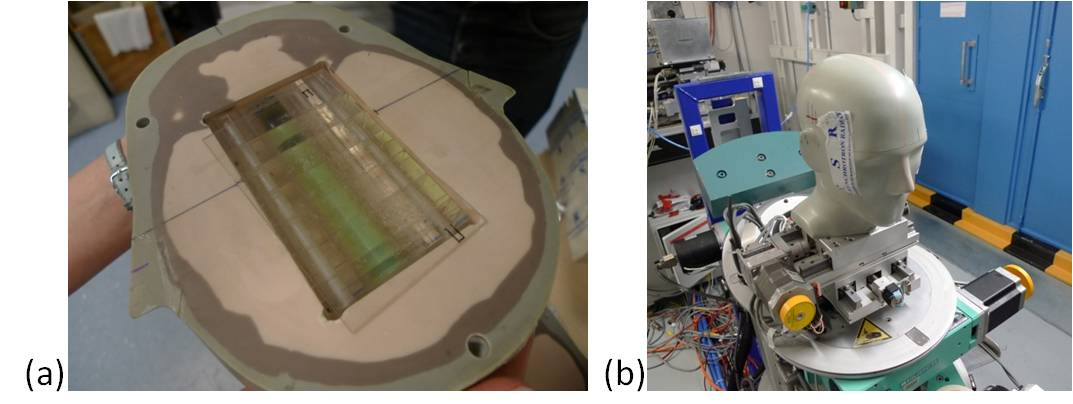
\includegraphics[width=0.9\linewidth]{Fig1}
\caption{(a) PRESAGE\textregistered \ sample 1.3 in place in anthropomorphic head phantom and (b) the head phantom being positioned for irradiation at the ESRF.}
\label{fig:Fig1christopher}
\end{figure}



\subsection{Results}
High quality image datasets were acquired for each sample and the microbeams are easily visualised. The reconstructed 3-D datasets can be visualised in different ways to provide an assessment of the irradiation. Figure~\ref{fig:Fig2MIP} shows a maximum intensity projection (MIP) image of a reconstructed image volume of sample 1.1, with the full dataset available in movie format as online supplementary material. This type of visualisation is very powerful, allowing the user to assess quickly that the pencil beam irradiation has been delivered successfully and is well centred within the sample. Confirming this would be very difficult using 2-D dosimeters. 

\begin{figure}
\centering
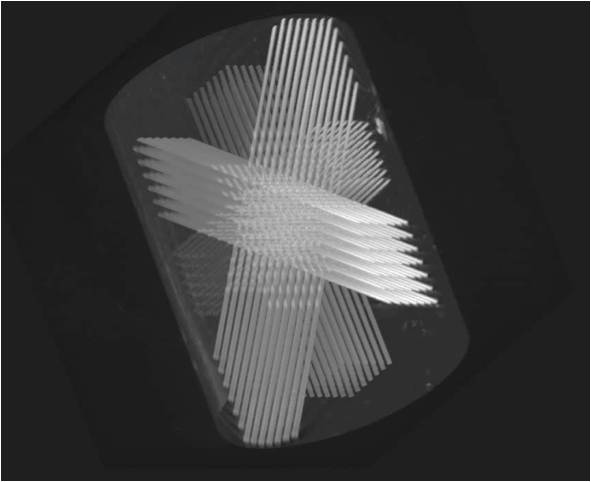
\includegraphics[width=0.7\linewidth]{Fig2}
\caption{A maximum intensity projection (MIP) image of sample 1.1 showing excellent visualisation of the microbeams, confirming successful irradiation which was well centred within the sample. Full 3-D reconstruction can be seen in video available online.}
\label{fig:Fig2MIP}
\end{figure}


Figure~\ref{fig:Fig3S9} shows a reconstructed slice through sample 1.2, irradiated with an interlaced dose pattern. More views are available in supplementary video material. It is clear that interlacing of the centre and left fields was successful. However, the centre and right fields are overlapping and the increased dose is visualised as a brighter region on optical CT images. This demonstrates the qualitative dose integration visualisation power of optical CT, which would be very helpful during MRT set-up even without a quantitative measure of the increased dose. This visualisation could inform on patient safety and would be complicated to measure with a 2-D dosimeter. 

\begin{figure}
\centering
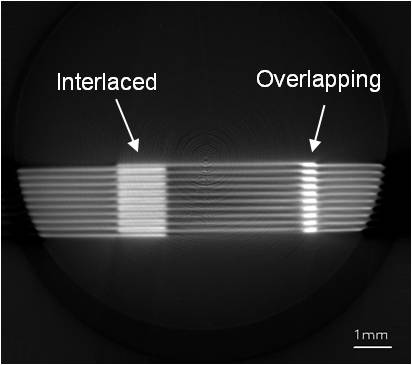
\includegraphics[width=0.7\linewidth]{Fig3}
\caption{A reconstructed slice through sample 1.2 with an interlaced dose pattern which has overlapped, leading to overdosing compared to the expected treatment. Further slices from the full dataset are available in a video online.}
\label{fig:Fig3S9}
\end{figure}


Figure~\ref{fig:Fig4L7} shows two orthogonal reconstructed slices through sample 1.3 which was irradiated inside an anthropomorphic head phantom with a multiport cross-firing geometry. With the ability to choose the image plane arbitrarily, it is easy to find a slice that gives direct interpretation of the delivered dose, unlike the image shown in Figure~\ref{fig:Fig4L7}(a). The second image, shown in Figure~\ref{fig:Fig4L7}(b), clearly shows that two of the delivered fields are off-centre and a simple measurement the offset could be used to correct the MRT geometry (red arrow). This interpretation would be very difficult from a 2-D measurement as the 2-D dosimeter would need to be placed very accurately. 


\begin{figure}
\centering
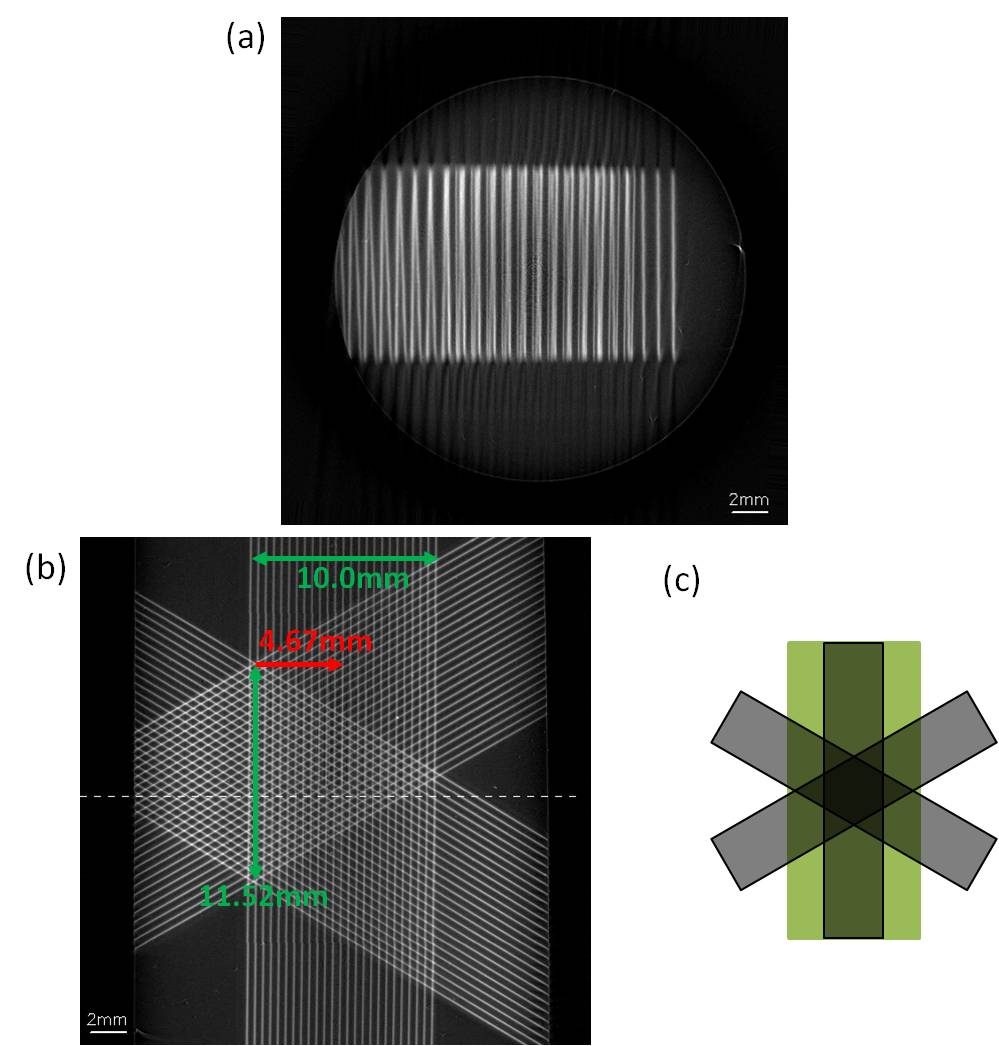
\includegraphics[width=0.9\linewidth]{Fig4}
\caption{(a) A reconstructed slice through sample 1.3 which was irradiated inside an anthropomorphic head phantom with a multiport cross-firing geometry. From this view it is difficult to tell whether the irradiation was successful. (b) A reconstructed slice in the orthogonal plane, with the z position of (a) marked by the dotted line. Green arrows mark field measurements which are as expected, showing that three irradiations have been delivered at the expected field size and spaced $60^{\circ}$ apart as expected. However, two of the fields are offset from the centre of the sample, (c) shows the expected shape of the irradiation. The red arrow denotes the offset of the two incorrect fields from the centre of the sample, this measurement could be used to correct the MRT geometry.}
\label{fig:Fig4L7}
\end{figure}




\section{Quantitative measurements of PVDR}
\label{sec:quantPVDR}
\subsection{Theory}
Previous publications have noted a reduction of optical CT image contrast of small features as the feature size approaches the resolution, resulting in an apparently different PRESAGE\textregistered \ dose response \cite{doranultra-high2013}. This effect is evident even when the feature size is several times the nominal spatial resolution and was thought to be an effect of the modulation transfer function (MTF). Therefore, it was important to characterise the MTF of our system over an extended depth-of-field (DOF) before making quantitative measurements of microbeams. 


\begin{figure}
\centering
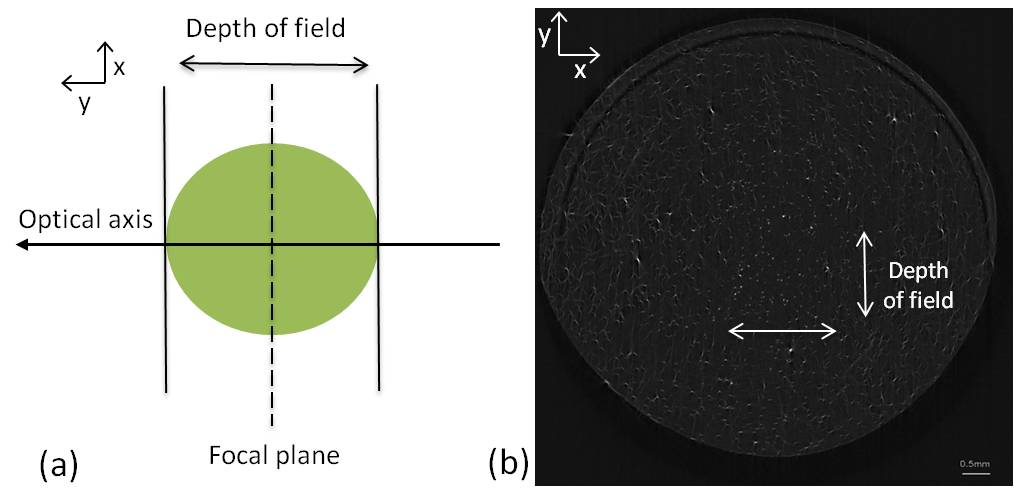
\includegraphics[width=0.9\linewidth]{Fig5}
\caption{(a) Ideal position of depth of field and focal plane for optical CT imaging. (b) Reconstructed image of a gel phantom containing 1$\mu$m beads demonstrating how limited depth of field in projection images affects reconstructed images.}
\label{fig:Fig5}
\end{figure}



Ideally the DOF of projection images should be larger than or equal to the sample size, as demonstrated in Figure~\ref{fig:Fig5}. However, there is a trade-off between DOF and resolution,  $\Delta x$, given by \cite{inoue1997video} as follows,
\begin{equation}
DOF = \frac{n_{bath}}{0.61 n \lambda} \big(\Delta x^2 + \frac{ne}{M_{lat}} \Delta x \big)
\label{eqn:1DOF}
\end{equation}

where, $n_{bath}$ is the refractive index of the medium surrounding the sample, $n$ is the refractive index of the medium around the lens, $\lambda$ is the wavelength of light, $e$ is the pixel size of the camera and $M_{lat}$ is the lateral magnification of the system. The DOF of the system can be adjusted by adjusting the overall acceptance angle of the system, $\theta$, which in turn controls the numerical aperture (NA) and this is inversely proportional to the resolution, 
\begin{equation}
NA = n \sin \theta = \frac{0.61n\lambda}{\Delta x}
\label{eqn:2NA}
\end{equation}

In a basic simulation of our system, we found that to measure the peak of a Monte Carlo-simulated 50$\mu$m microbeam with an error of less than 1\%, a sampling resolution of $10\mu$m is required. Therefore, the optimum NA giving this resolution over the largest DOF needs to be found.  

One method of measuring the resolution of a system is to obtain the MTF, which measures how well the system can transmit spatial frequencies. This can be calculated by taking the Fourier transform of the derivative of the edge-spread function (ESF), 
\begin{equation}
\mathrm{MTF}(f)  = \mathcal{F}\left[\frac{d}{dx}\mathrm{ESF}(x)\right]
\label{eqn:3MTF}
\end{equation}
where the ESF can be measured using a knife-edge test object (see \cite{chenincorporation2012} for details). 

\subsection{Methods}
\subsubsection{Depth of Field characterisation}
A series of experiments similar to those performed by \cite{chenincorporation2012} was undertaken to characterise the DOF of the optical CT system for different NA values. The NA is controlled through an aperture in the Leica lens system of our optical CT microscopy scanner. The aperture can be set to five repeatable sizes, labelled A1 (smallest NA) to A5 (largest NA).

A knife edge was positioned at the focal plane and 50 projection images of matrix size $2048 \times 2048$ were acquired and averaged to improve the SNR. The knife edge was moved in steps of 0.1mm away from the focal plane in both directions along the optical axis. Images were acquired over a distance of 0.5mm in each direction giving a total distance of 10mm, the same as the FOV of each projection image. This was repeated for five different NA settings of the microscope lens, A1−A5.

The MTF was calculated from the ESF, measured across the centre of the knife-edge images, according to equation~\ref{eqn:3MTF} for each position along the optical axis and for each NA value. The MTF was represented by a grey level in a 2-D image in which the horizontal coordinate corresponds to spatial frequency, up to the desired 100mm$^{-1}$ (equivalent to a $10\mu$m line-pair), and the vertical coordinate corresponds to position along the optical axis. This allows visualisation of the DOF for each of the different NA values.
The maximum resolution and corresponding DOF were measured for each NA setting. The maximum resolution was defined as the largest spatial frequency with an MTF above 10\% at the focal plane. The DOF for this frequency was defined as the distance along the optical axis for which this spatial frequency had an MTF above 10\%.  

\subsubsection{PVDR measurement}
PRESAGE\textregistered \ samples were irradiated with microplanar arrays of different field sizes and different peak doses to provide a range of PVDRs for comparison with Monte Carlo and film data. Samples were laid in the phantom and exposed end-on to a single irradiation from a multi-slit collimator of slit width 50$\mu$m, centre-to-centre spacing 400$\mu$m \cite{brauer2009new}. Two 9.7mm diameter samples were exposed with a nominal peak dose to the surface of the dosimeter of 50Gy and 100Gy, both with a field size of $(10 \times 10)$ mm$^2$ (samples 2.1 and 2.2 respectively). A third 9.7mm sample was exposed with a nominal peak dose of 100Gy, with field size ($30 \times 30$) mm$^2$ (sample 2.3, see Table~\ref{table:samples}). 

Samples 2.1−2.3 were scanned using a `high-resolution' scan consisting of 3300 projections, each averaged over five acquisitions of 2048 $\times$ 256 pixels, reconstructed to a data volume of 2048 $\times$ 2048 $\times$ 256 voxels with FOV (10 $\times$ 10 $\times$ 1.25) mm. Using the full matrix size of the new camera across the width of the sample allows significantly higher sampling frequency over previous reports, with an isotropic reconstructed voxel size of (5.2 $\mu$m)$^3$. A smaller matrix height of 256 pixels was chosen for reduced acquisition and reconstruction times. The large computer RAM of 256 GB allows readout of the large amounts of data simultaneously making these scans a manageable 1 hour long. The projections were acquired with the largest DOF setting (smallest NA, setting A1), reflecting the `ideal' focal situation of constant resolution across the entire sample. The samples were scanned at depths of 0.3cm, 1cm and 4cm for comparison with Monte Carlo and film measurements of PVDR \cite{martinez-roviradevelopment2012}. 

\subsubsection{Deconvolution}
Using a high NA would give a high resolution at the cost of a small DOF, resulting in out-of-focus data being superimposed on top of in-focus data requiring deconvolution. To investigate whether the resolution could be improved through deconvolution with a measured point-spread-function (PSF), a PSF phantom was designed. The PSF phantom was made using 1$\mu$m diameter beads (56314, Sigma-Aldrich) which were suspended in 0.75\% agarose gel. The gel was dehydrated in 100\% ethanol and then soaked in matching fluid (97\% ethyl hexyl salicylate and 3\% 4-methoxycinnamic acid 2-ethylhexyl ester) giving the same refractive index as the PRESAGE\textregistered. Superglue was used to attach the bead phantom to the end of PRESAGE\textregistered \ sample 2.1. The bead phantom was then included in the FOV during a `high-resolution' scan consisting of 3300 projections, each averaged over five acquisitions of 2048 $\times$ 256 pixels, reconstructed to a data volume of 2048 $\times$ 2048 $\times$ 256 voxels with FOV (10 $\times$ 10 $\times$ 1.25) mm. The lens aperture was set to A4  which had the largest DOF for 10$\mu$m resolution (see Table~\ref{table:DOFNA}). 

When images were reconstructed, in principle a bead at point (x, y, z) has experienced the same optical blur as at point (x, y, z + $\Delta $z). Assuming this, a bead in the centre of the sample in good focus was used as a PSF during Richardson-Lucy deconvolution of the microbeam profile axially above it at a depth of 0.3cm in PRESAGE\textregistered. Deconvolution was performed in the IDL software environment (Exelis Visual Information Solutions, Boulder, CO) using the `deconv' tool \cite{varosi1993idl}, assuming Poisson noise. The PVDR from the resulting deconvolved profile was calculated for different numbers of deconvolution iterations.

\subsection{Results}
\subsubsection{Depth of field characterisation}
The results of knife-edge measurements of the MTF over an extended DOF are shown in Figure~\ref{fig:Fig6}. These results show that with NA setting A1, the ideal situation of a constant resolution across the entire FOV is broadly achieved. However, the maximum resolution is only $21.5 \pm 0.5\mu$m. A resolution of 10$\mu$m is achieved when the NA is increased at an aperture setting of A4, but in this case, the DOF less than 0.6mm (see Table~\ref{table:DOFNA}).

\begin{figure}
\centering
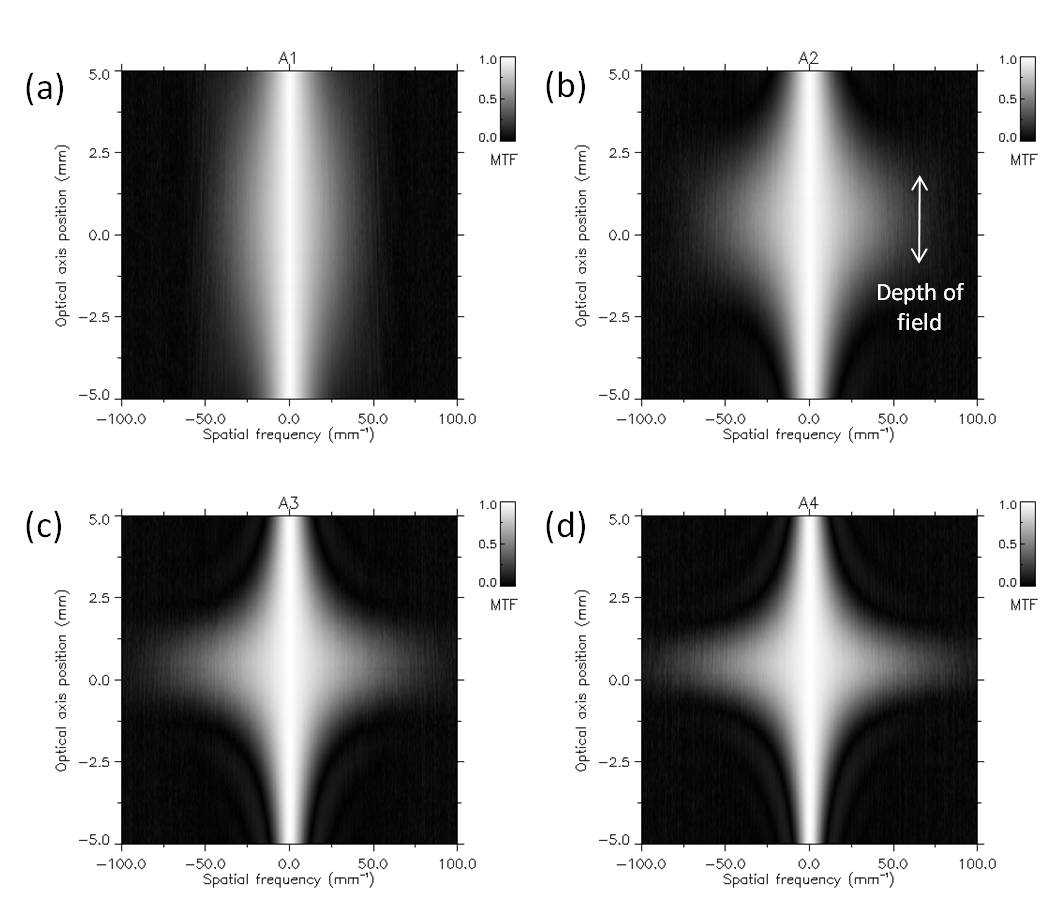
\includegraphics[width=0.9\linewidth]{Fig6}
\caption{Measurements of the modulation transfer function (MTF) along the optical axis for different numerical aperture (NA) settings of the system, (a) A1 (b) A2 (c) A3 (d) A4. This allows visualisation of the depth-of-field (DOF).}
\label{fig:Fig6}
\end{figure}

\begin{table}[H]
	\centering
	\begin{tabular}{ p{2.5cm}  p{3.5cm} p{4.5cm}  }
		\hline
		\textbf{NA setting} & \textbf{Resolution ($\mu$m)} &\textbf{Depth of field (mm)}  \\ \hline
		A1  & $21.5 \pm 0.5$ & $9.3 \pm 0.4$ \\ %\hline
		A2  & $13.7 \pm 0.1$ & $2.4 \pm 0.2$ \\ %\hline
		A3  & $12.0 \pm 0.2$ & $1.6 \pm 0.2$ \\ %\hline
		A4  & $10.1 \pm 0.2$ & $0.6 \pm 0.1$ \\ %\hline
		A5  & $9.7 \pm 0.2$ & $0.4 \pm 0.1$ \\ \hline		
	\end{tabular}
	\caption{Maximum resolution and corresponding depth-of-fields for different NA settings on the optical CT system. The uncertainties reflect noise in the modulation transfer function (MTF)  measurements.}
	\label{table:DOFNA}
\end{table}


\subsubsection{PVDR measurement} 
Figures~\ref{fig:Fig7}(a) and (b) show a reconstructed optical CT image of PRESAGE\textregistered \ sample 2.1 and the associated profile through the marked position on the image. To reduce noise, profiles were median-averaged in the two orthogonal directions to the microbeam variation resulting in an effective pixel size of 104$\mu$m in those directions and 5.2$\mu$m across the profile. Over this small distance there is no divergence of the peak pixel position in the orthogonal directions as the beam divergence is very small. 

As no part of the sample was unirradiated, the baseline corresponding to zero-dose pixel value used is an average of values obtained from unirradiated areas of other samples from the same batch, hence the large uncertainty marked on the graph. In future a pre-scan can reduce this error. As can be seen the sampling frequency is very high, however the beams appear blurred compared to the shape observed with other higher-resolution modalities. 

The PVDR was calculated for sample 2.1 at depths of 0.3cm, 1cm and 4cm. Samples 2.2 and 2.3 were also measured at a depth of 4cm. The results of the optical CT PVDR measurements are plotted against the expected values from Monte Carlo simulation \cite{martinez-roviradevelopment2012} in Figure~\ref{fig:Fig7}(c), where the large error-bars on the optical CT measurements are principally due to the baseline uncertainty. Encouragingly, the variation of PVDR with depth and field size corresponds extremely well between optical CT and Monte Carlo measurements with a very high correlation coefficient for the linear fit. However, the absolute value of the PVDR, as measured by optical CT is consistently only 30\% of the expected value. There could be several reasons for this. Given that decreasing the peak entrance dose has no effect (sample 2.2) it is unlikely to be due to a lack of dynamic range in the optical CT scanner. Sample 2.3 has a larger field size and therefore larger valley dose. Given that this measurement also fits the trend it is unlikely that low SNR in the valley measurement is the primary source of the error. 

The full-width half-maximum (FWHM) of one of the beams in Figure ~\ref{fig:Fig7}(b) is 62.4$\mu$m, not 50$\mu$m as expected. This implies that the profile is blurred, which would reduce the peak value measured. Although the nominal pixel size is 5.2$\mu$m, the true resolution is lower than this, limited by the imaging optics, as expected from our MTF measurements. 

\begin{figure}
\centering
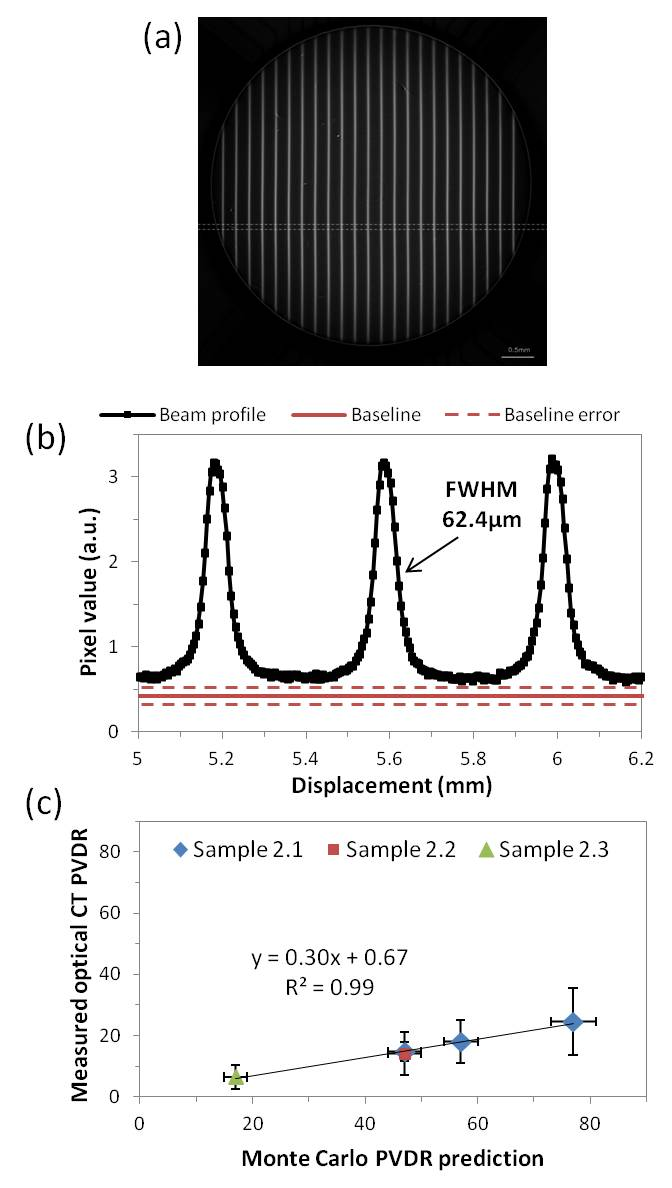
\includegraphics[width=0.6\linewidth]{Fig7}
\caption{(a) Reconstructed image of sample 2.1 and (b) the corresponding profile through microbeams. The baseline is an average value from unirradiated areas on other samples from the same batch, hence the large uncertainty. The profile was median averaged along 20 pixels in the directions orthogonal to the profile to improve the SNR resulting in 5.2$\mu$m pixel size across the profile and 104$\mu$m pixel size in the orthogonal directions. (c) Comparison of PVDR measurements using optical CT against expected values from Monte Carlo simulation \cite{martinez-roviradevelopment2012}.}
\label{fig:Fig7}
\end{figure}



\subsubsection{Deconvolution}
Figure~\ref{fig:Fig8}(a) shows a microbeam profile and its improved shape after deconvolution with a PSF measured using a 1$\mu$m diameter bead. However, Figure~\ref{fig:Fig8}(b) clearly demonstrates that although the deconvolution improves the shape of the profile, the PVDR measured is dependent on the number of deconvolution iterations performed, and does not converge before the noise reaches an unacceptable level. This means that this type of deconvolution approach is not reliable enough to use in quantitative measurements of PVDR of microbeams. This may also apply to depth-of-field scanning techniques previously employed in biological imaging to improve the resolution \cite{fauverthree-dimensional2005}. 

\begin{figure}
\centering
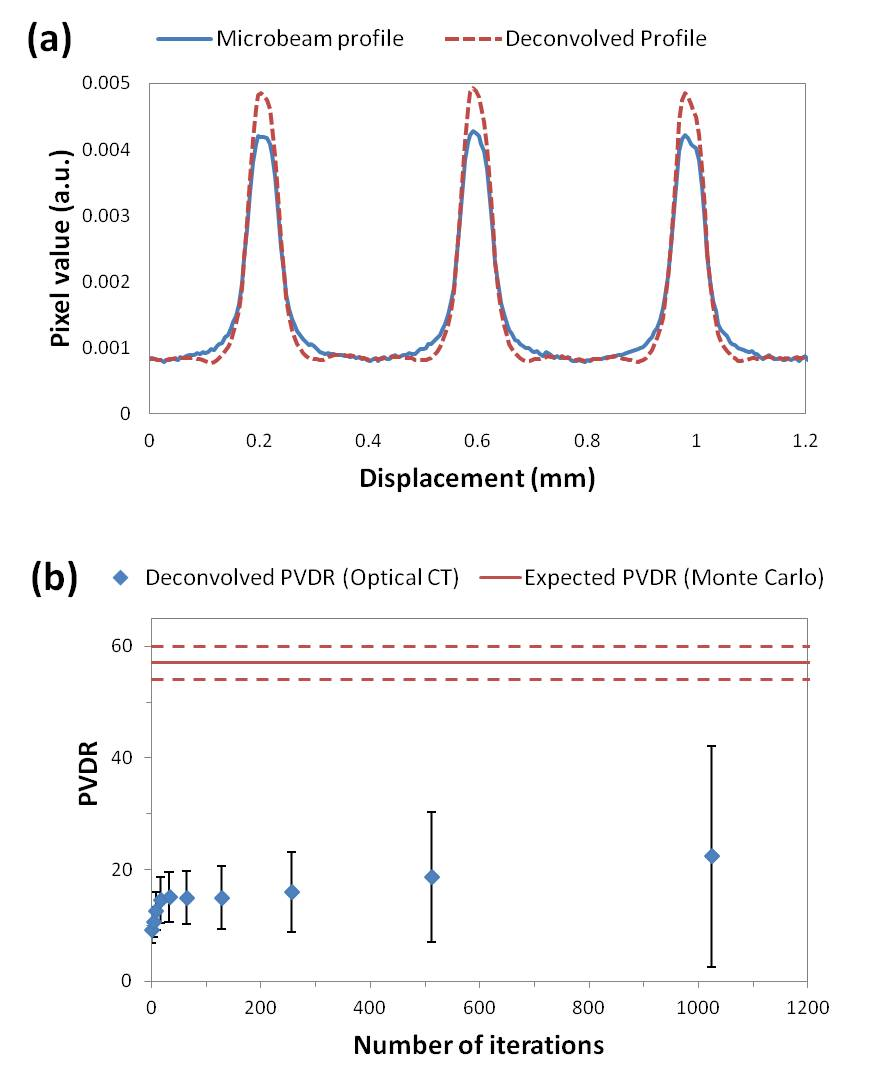
\includegraphics[width=0.85\linewidth]{Fig8}
\caption{(a) A microbeam profile from sample 2.1 and the deconvolved profile after 4 iterations of Richardson-Lucy deconvolution using a PSF calculated from a 1$\mu$m bead. This shows that deconvolution of the PSF improves the shape of the profile however, (b) shows that the PVDR depends on the number of deconvolution iterations, which does not appear to converge before becoming extremely noisy. Therefore although deconvolution can qualitatively improve the images, we are hesitant to base any quantitative measurements on a deconvolved profile.}
\label{fig:Fig8}
\end{figure}


\section{Discussion}
Section~\ref{sec:3dvis} clearly suggests that optical CT has the potential to play an important role in MRT QA. The data of Figures~\ref{fig:Fig2MIP}-\ref{fig:Fig4L7}, rendered in 3-D in the accompanying movies, demonstrate graphically where the real benefit of the optical CT technique lies. Image data may be acquired from the entirety of the sample at high resolution in a single measurement. This would be very useful for hit-or-miss assessment and imaging is now fast enough to provide correction information to improve MRT irradiations \textit{in situ}. Compared with a single, or small number of 2-D film images, there are no difficulties in interpreting the measured dose distribution in multiport treatments. Using the solid PRESAGE\textregistered \ dosimeter also allows for end-to-end QA of the entire treatment process including CT scan, treatment planning, positioning and delivery which would be necessary before MRT is translated to clinical use. One potential future application would be to combine PRESAGE\textregistered \ dosimetry with a patient motion simulating platform which can investigate whether very complex irradiations such as interlacing are possible with patient breathing motion. 

The time between irradiation and readout was longer than desirable, during which time the samples were refrigerated. The potential time-evolution of the measured doses is discussed in \cite{doranestablishing2013} but whilst the error introduced at this step is expected to be significant, the pertinent observation for the purposes of this work is that PRESAGE\textregistered \ exhibits negligible diffusion of the dose-reporting chromophore. Thus, blurring of the microbeam dose due to the delay is not expected to have occurred.
 
The apparatus is sufficiently compact that a copy could be installed in the MRT hutch at ID-17. A number of improvements to the imaging methodology would be possible if the apparatus were located in situ at the beamline:
\begin{itemize}
	\item As was discussed in \cite{doranestablishing2013}, pre-scanning the dosimeter would enable effects of refraction to be largely eliminated and an accurate zero-dose baseline to be established, for absolute measurements of valley dose given the new accurate positioning system.
	\item Images could be acquired within minutes of the end of the irradiation, eliminating any uncertainties caused by delayed readout, for example, related to time-evolution of the PRESAGE\textregistered \ dose-response \cite{skyttemperature2011 , skyttemperature2012}.   
	\item Further improvements in image SNR and extensions to the dynamic range of acquired data would be achievable via the acquisition of multiple datasets with different levels of illumination \cite{krstajiccharacterization2007 , thomasa2011}.
\end{itemize}


The results of Section~\ref{sec:quantPVDR} suggest that accurate PVDR measurements are not possible with the current optical CT arrangement. Given the results of the knife-edge measurements of MTF along the optical axis, we believe the underestimation of the PVDR by optical CT is primarily due to lack of true spatial resolution. Attempts to improve the resolution by increasing the numerical aperture and deconvolution using a measured PSF lead to unreliable and noisy results, making these methods unsuitable for clinical measurements of PVDR.   

It remains an open question as to whether the optical CT technique will in future prove capable of making measurements of PVDR that are competitive with other methods such as those employing 2-D TLD films or MOSFET detectors. There are two possible avenues to move forward with quantitative microbeam measurements using optical CT. 

First, using a smaller sample would mean that both the necessary FOV and DOF can be decreased, making it possible to increase the magnification and resolution. Although this involves the sacrifice of spatial information across the beams, full depth information would still be retained. This would enable, among other things, measurement of the effects of scattering along the entire length of the microbeams, rather than simply at a single depth determined by the detector location. 

Second, while the measured resolution of $21.5 \pm 0.5 \mu$m in projections with NA setting A1 is insufficient for sampling the peak dose, it should be sufficient for quantitatively measuring the valley dose, which is four times wider than the peak. Arguably, in terms of patient safety the valley dose is the most important factor, as once the peak is over a certain value, cell death will occur. Therefore, having a valley measurement in 3-D, in combination with an alternative 2-D measurement of the peak dose on entry, could be of significant interest to the MRT community.

\section{Conclusions}
3-D images of geometrically sophisticated synchrotron microbeam therapy deliveries have been obtained. The most significant current limitation of the imaging technique as presented here is the available spatial resolution, which has been investigated in detail. Although the data presented here fall some way short of the dose quantification needed for complete verification, the measurements and visualisations have already demonstrated their utility by detecting deviations from a planned treatment (Figures~\ref{fig:Fig3S9}, \ref{fig:Fig4L7}(b)) and shown clear potential for quantitative measurement of the biologically important valley dose.





\bibliography{readcube_export_mrt}

\end{document}